\documentclass{article}

\usepackage{fullpage}
\usepackage{graphicx}
\usepackage{hyperref}
\usepackage{longtable}

\newlength\tindent
\setlength{\tindent}{\parindent}
\setlength{\parindent}{0pt}
\renewcommand{\indent}{\hspace*{\tindent}}

\title{Web Technologies: Report}
\author{Jannick Hemelhof, Roberto Ristuccia, Youssef Boudiba}

\begin{document}

\maketitle
\newpage
\tableofcontents
\newpage
\pagenumbering{arabic}

\section{Introduction}
Do you like taking pictures of strange things that happen around us? Do you want to share it with your friends, family and other people with the same passion? If you answered yes on all those questions then you will surely love the website we created. Add new sightings while marking the location where it took place. Watch sightings posted by other people and comment to start a discussion. Search through our database for a specific sighting, visit the profiles of other UFO spotters and get in touch! So why are you still reading this? Let's collect those strange sightings!

\section{Design}
For the project we made use of the so called MEAN stack. This stack incorporates following components:
\begin{itemize}
\item MongoDB, a NoSQL database
\item Express.js, a web application framework that runs on Node.js
\item AngularJS, a JavaScript MVC\footnote{ Model-View-Controller} framework that runs in browser JavaScript engines
\item Node.js, an execution environment for event-driven server-side and networking applications
\end{itemize}
We picked this application stack because it let us program client and server side in the same language, being JavaScript. 
As for the architecture of the stack, Figure 1 shows how the different parts of the stack work together.
\begin{figure}[hb]%                 use [hb] only if necceccary!
  \centering
  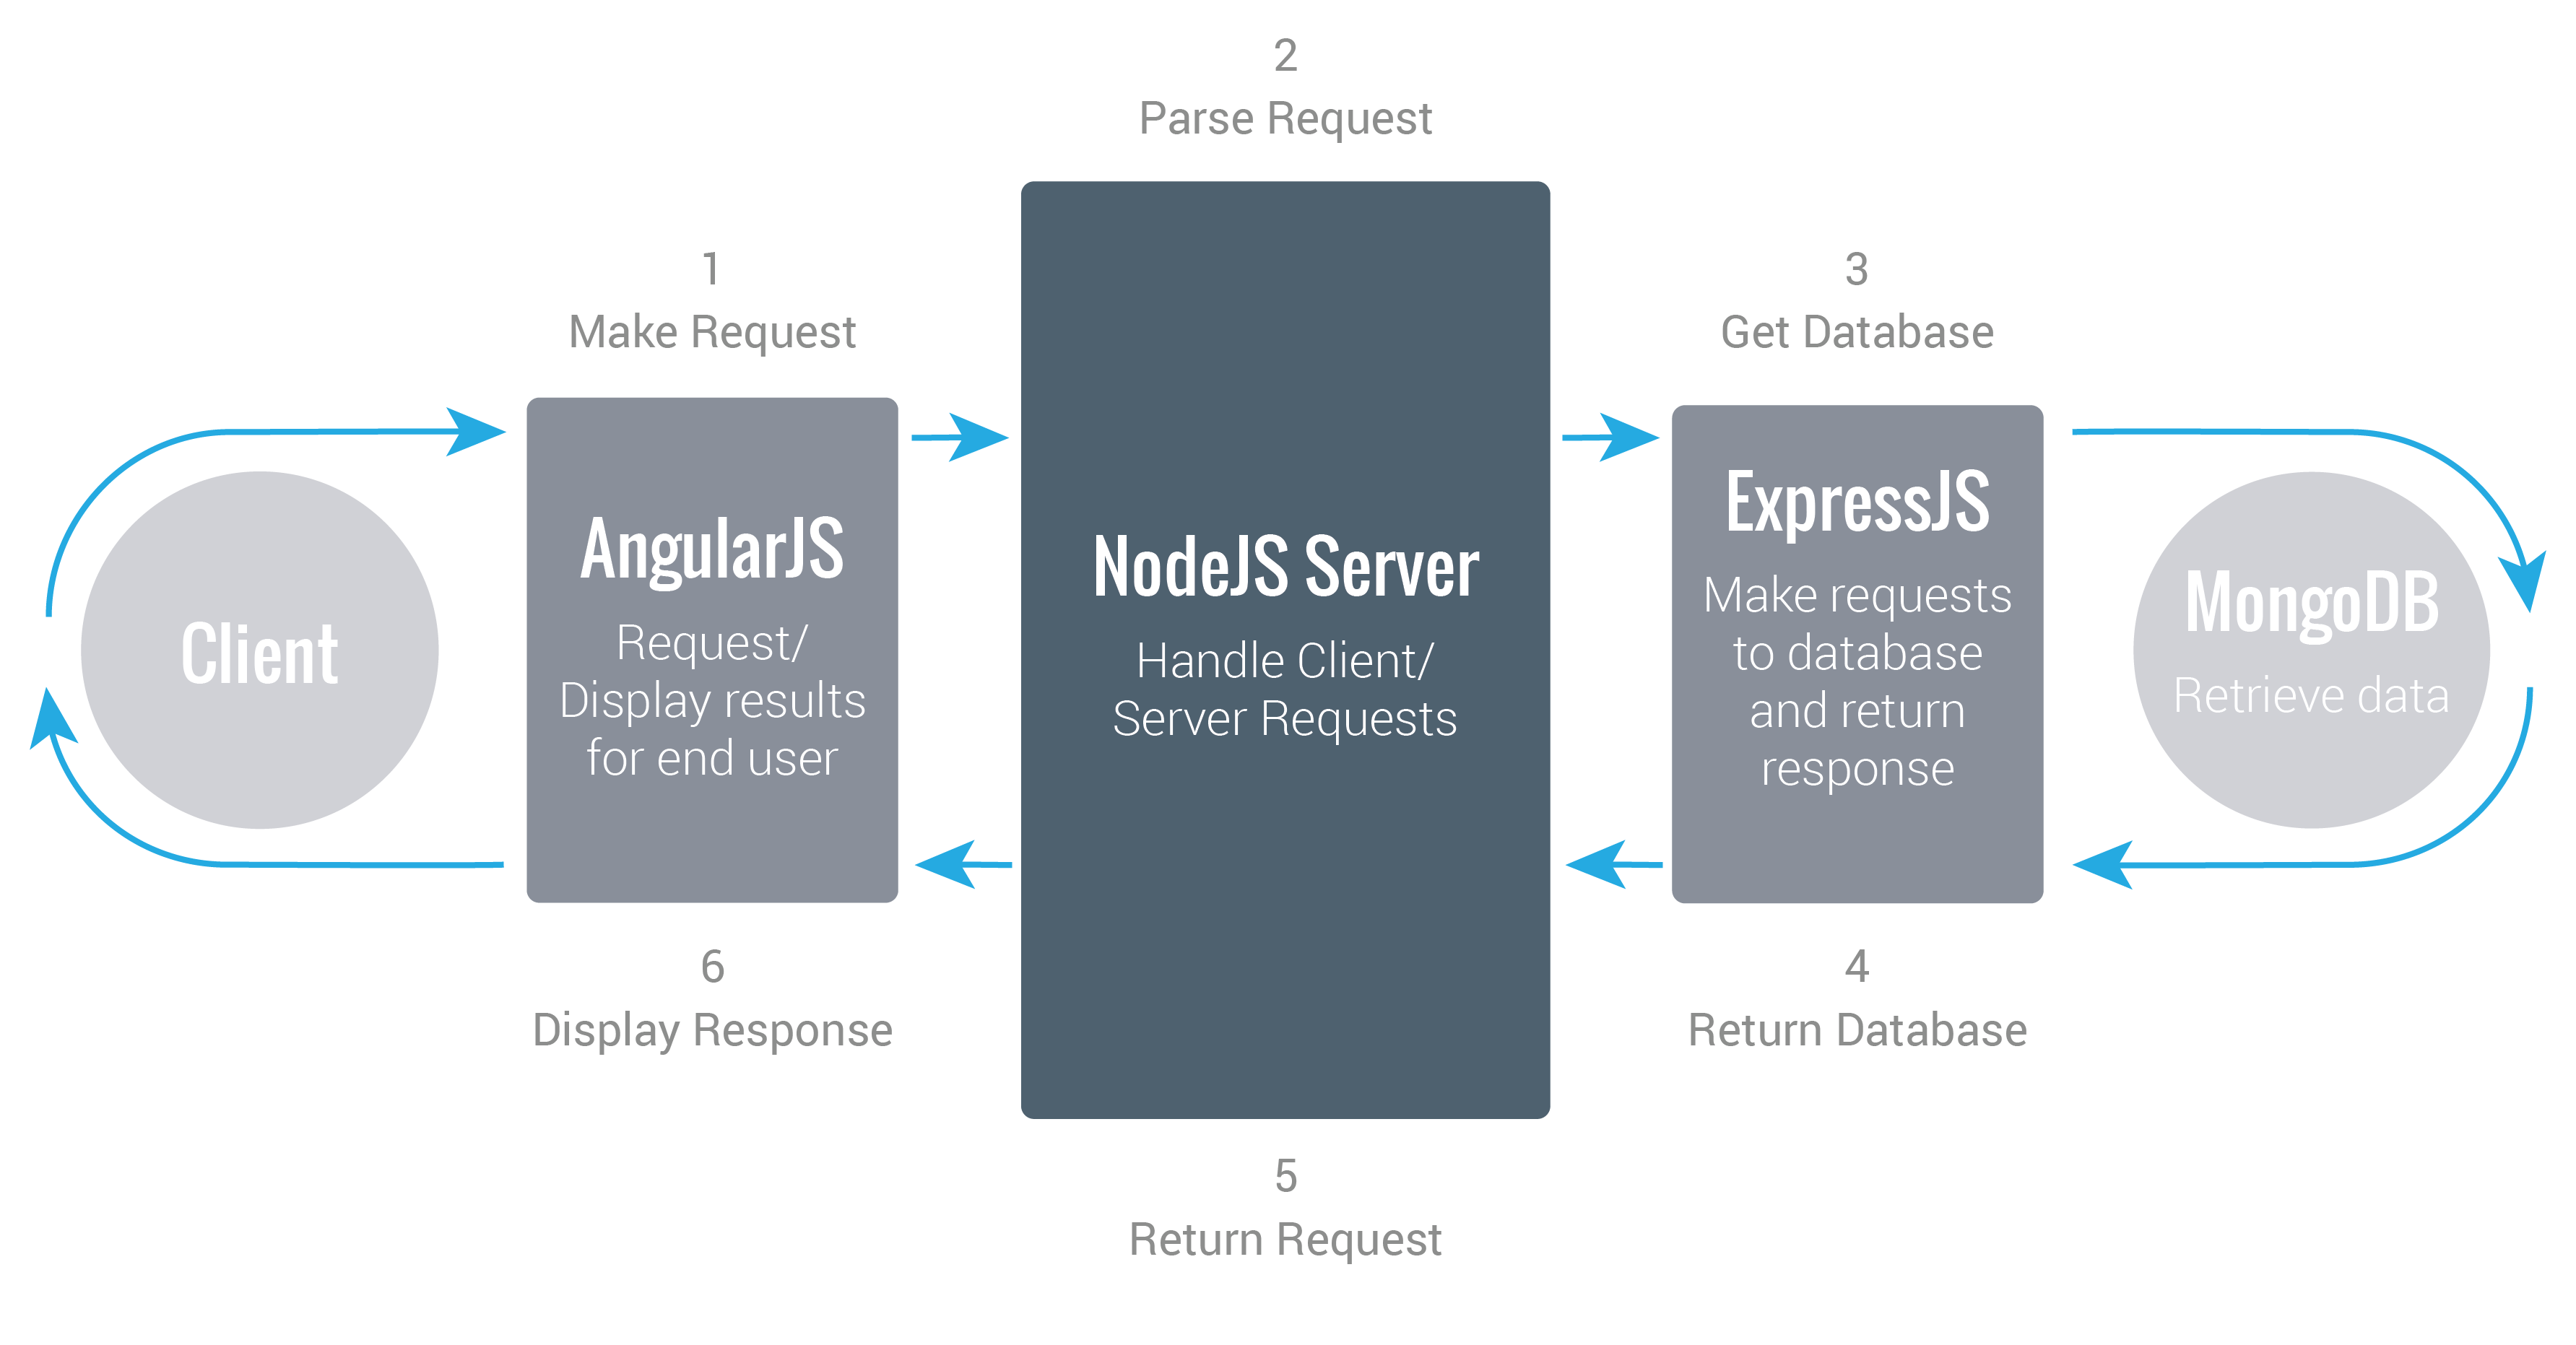
\includegraphics[width=15cm]{architecture}
  \caption{Image source: \url{http://lgitsmart.com/2015/02/25/mean-one-language-to-rule-them-all/}}
  \label{fig:test}
\end{figure}

\section{Handling of Requirements}
\subsection{User can register}
Users need to register themselves first in order to be able to log in into the system. This happens on the signup page. Whenever users register themselves, two kind of check-ups take place. On one hand we have client-side validation of the form (username, password and e-mail), which is done by HTML5 validators (more information on that in section 3.5). On the other hand we have server-side validation which ensures that the username is not already taken. \\

Once the user has filled in all the fields (and the username is not taken), he can press the signup button which will fire an angular \$http post request with the filled form as parameter.
Server-side the form is intercepted and if everything goes well (username not taken) a new user is created in the MongoDB database. As a result, a json-web-token is generated and send back to the client where it will be stored in the Local Storage. The token is used for session management and will remain valid for 24 hours after which it needs to be refreshed. \\

If everything goes well the user will be logged in and redirected to the "UFO Sightings" page.

\subsection{User can log in}
In order to post new sightings  or comments in the sighting database, users must be logged in. The process of logging in to the system works the same way as the process of registration. In fact, we also have client-side and server-side validation of the filled form. The difference here is that at server side we actually check whether or not a username exist and if so we make sure that the password associated is correct. Only then can a user log in and like the registration he will be redirected to the sightings page. \\

When the user press the login button, it fires an angular \$http post request with the filled form (username \& password) as parameter. A "new" user is created server-side and the server responds with a json web-token. \\

The user is now connected or has logged in and is redirected to the "UFO Sightings" page.

\subsection{User has a profile}
When registering you need to enter an e-mail and a username. This was done from with privacy in our mind: a user shouldn't be forced to provide any other info if he doesn't want to. If you're logged in you can visit your profile and expand it. Pressing the "Edit Profile" button lets you enter a first- and last-name. Changing your e-mail is also a possibility. \\

Keep in mind that you can't change your username: it's unique and should stay that way.

\subsection{User can manipulate data}

\subsubsection{Sightings page}
Connected users and guest users can view a list of all the sightings on the "UFO Sightings" page. Of course only connected users can post new sightings and comments. The sightings page shows a list of all sightings present in the database and makes sure recently added sightings are shown first. \\

Whenever a user visit the "UFO Sightings" page, an \$http get request is triggered which will retrieve all the sightings from the database.

\subsubsection{Search for a sighting}
(Guest) users can search for a specific sighting by making use of the search box present in the navigation bar. First all sightings are retrieved from the database via an \$http get request. After that a filter is applied which will filter out the relevant sightings.

\subsubsection{Add new sighting}
As mentioned earlier, only connected user can post new sightings. This happens on the "UFO Sightings" page by pressing the "Post a new sighting" button. A modal form will pop up. The user will be asked to fill in all necessary information (title, description, etc.). Form validation occurs on client side. If a user doesn't upload a picture, a default will be chosen instead. Same goes for the location. \\

All that's left is to press the "New Sighting" button, which will fire an angular \$http post request with the filled form and the json web-token as parameter. At the server-side additional information will be added to the form, such as a unique ID and the date the sighting has been posted. Now all that's left is to save the sighting in the database.

\subsubsection{Edit and delete sightings}
Any logged-in user can edit and/or delete his sightings. This happens on the profile page. A list of the user's sightings will be shown along with two buttons: "edit" and "delete". Currently only the title and description can be edited. Deleting the sighting from the database only require to press the delete button. \\

The way this works is pretty straightforward. 
First the user gets all his sightings via an \$http get request with the username as parameter. The server responds with a list of all the user's sightings. 
Whenever a user press the edit button on a specific sighting a modal form pops up. Now the user can edit the title and the description of the sighting. After applying some modifications the user can press the "Edit Sighting" button which will fire an angular \$http put request with the new form and the user's json web-token as parameter. At server-side the modifications are applied.
As mentioned above, deleting a sighting only requires the user to press the delete button, which will trigger an angular delete request with the token and the sighting as parameter. At server-side the right sighting is looked up via it's ID and deleted.

\subsection{Social aspect is needed}
Logged in users can leave comments on each sighting, that way they can interact with other users. This makes the website fun to use. Comments are visible for everyone, even guests so if you don't understand something and post a comment to ask for more information the whole internet will know it!

\subsection{Usage of AJAX}
Using AJAX is trivial thanks the http service from AngularJS. Sending requests via this service returns a so called 'promise' object with two functions: success() and error(). Calling these functions permits us to choose what will happen when the AJAX call finishes.
With this service working behind the scenes we can use all the advantages of AJAX in our website:
\begin{itemize}
\item Posting a new sighting: New sighting shows up without reloading the page
\item Updating user profile: Updates are immediately visible
\item Updating sighting: Updates are immediately visible
\end{itemize}
AJAX permits us to only force a refresh when there's no other option. Thanks to that we can provide a much smoother user experience.

\subsection{Form validity}
While thinking about handling this requirement our initial thoughts saw form validation as something that would happen on the server side of our application. Rereading the assignment gave some other insights and discovering the very neat validator.js\footnote{ Validator, for Bootstrap 3: \url{http://1000hz.github.io/bootstrap-validator/} } library showed us that client side validation could look good and was straightforward to implement.
\begin{itemize}
	\item Server side: We have built in some checks that ensure a consistent status of our database: When registering a username needs to be unique and the required fields need to be filled out. The check for required fields is also present on the client side but since someone can manipulate requests to maybe remove some data after the client side check an insurance policy was needed on the server side. These checks for required fields are present all over the server side where data is being received.
	\item Client side: We added some basic checks: Required fields need to be filled out and, by using the HTML5 input fields, designated input fields need to have a value that corresponds with the type of field. When there is an error (e.g. a required field wasn't filled in) the field is marked and an error is shown explaining what the problem is. This is possible thank to the validator.js library.
\end{itemize}

\subsection{CSS + Responsive Design}
While designing our website we realised that the most likely device to post a new sighting on is a mobile device. You're walking around, you see something and want to post it right away. That's why we needed a mobile friendly design, and CSS is really our friend for this. \\

We chose not to reinvent the wheel and picked the bootstrap framework\footnote{ Bootstrap, \url{https://getbootstrap.com/}} as our desired tool to use.
We incorporated the Bootstrap elements throughout our HTML files and tested it on a wide range of mobile devices (smarthphone, tablets, ...) and not only was it easy to use it also provided a consistent user experience across these devices. Risking that our website would look the same like other groups - who were also using Bootstrap - some personal CSS was added to provide a unique look and feel to our project.

\subsection{HTML5 features}
For this requirement we went ahead and implemented following HTML5 specific features:
\begin{itemize}
\item Local Storage: In order to remember the logged in user across different sessions we're using the local storage feature to place a token. That way we can check if there's a user logged in at the moment.
\item Geolocation: A user who has just seen a UFO out in the field might be too shocked to remember where he is at the moment. By using the HTML Geolocation API we can just use the location of the device on use that data when submitting the sighting.
\item Notification: Showing the user that an operation was successful would be possible by letting a custom form/modal pop up but we were aiming for a more native solution. By using the Notifications API (supported by Chrome, Firefox, and Safari) we can offer the user a confirmation that his request was handled in a native environment.
\item Input fields/Validators: In our input forms we use some new HTML5 input types e.g. email but also the required attribute.
\end{itemize}

\subsection{Web Services}
Our initial idea was to provide weather data for each sighting. Sadly, we realised that weather data is mostly aimed at forecasting and not at historical information for a specific date. We then decided to Imgur API\footnote{The Imgur API: \url{http://api.imgur.com}} since our goal from the start was the ability for the user to upload an image when posting a sighting.  Hosting images ourselves isn't really scalable so using this external web service helps us a lot.
Usage of the Imgur API happens on two occasions:
\begin{itemize}
\item Home page: When a user lands on our homepage, we sent a GET request to the API in order to receive 50 images taken from the UFO gallery. That way we can show the user something interesting but also relevant. That way we might have even room for sponsored images.
\item New Sighting: When posting a new sighting a user should be able to provide an image of what he/she has just seen. As said before, we're not interested in hosting these images ourselves so that's where the angular-imgur-upload\footnote{Angular.js Imgur Upload service: \url{https://github.com/purple-circle/angular-imgur-upload}} library comes in. After the user has selected an image to upload, we use this library to sent it to Imgur. We then save the url to the image in our sighting, a url we get from the response of the Imgur API.
\end{itemize}

\subsection{Provide data}
Providing our data so others can use it is a straightforward and easily accomplished task. We went further with that idea and provide a simple API so developers can develop their own applications for managing UFO sightings using our infrastructure. We support following commands:
\begin{center}
    \begin{longtable}{ |  l  |  l  |  l  |  p{2cm}  |  p{2.6cm}  |  p{3cm}  | }
    \hline
    Idea & Type & Path & Auth header & Parameters & Return value \\ \hline
    Register a user & POST & /signup & no & \begin{itemize}
    \item username
    \item password
    \item email
\end{itemize} & \begin{itemize}
\item auth token
\end{itemize} \\ \hline
    Login a user & POST & /login & no & \begin{itemize}
    \item username
    \item password
\end{itemize} & \begin{itemize}
\item auth token
\end{itemize} \\ \hline
    Get user info & GET & /user & no & \begin{itemize}
    \item username
\end{itemize}     & \begin{itemize}
\item username
\item email
\item firstname
\item lastname
\end{itemize} \\ \hline
    Update user info & PUT & /user & yes & \begin{itemize}
    \item username
    \item email
    \item firstname
    \item lastname
\end{itemize}     & \\ \hline
Get sightings & GET & /sightings & no & & \begin{itemize}
\item sightings
\end{itemize} \\ \hline
Add sighting & POST & /sightings & yes & \begin{itemize}
\item title
\item description
\item day
\item month
\item year
\item url
\item coordinate
\item author
\end{itemize} & \\ \hline
Post comment & POST & /comment & yes & \begin{itemize}
\item content
\item author
\item sightingID
\end{itemize} & \\ \hline
Get sighting & GET & /sighting & no & \begin{itemize}
\item sightingID
\end{itemize} & \begin{itemize}
\item sighting
\end{itemize} \\ \hline
Update sighting & PUT & /user/sightings & yes & \begin{itemize}
\item sightingID
\item title
\item description
\item date
\end{itemize} & \\ \hline
Delete sighting & DELETE & /user/sightings & yes & \begin{itemize}
\item sightingID
\end{itemize} & \\ \hline
    \end{longtable}
\end{center}

\subsection{Google Maps}
We used the Google Maps API on two occasions:
\begin{itemize}
\item New sighting: When a user is reporting a new sighting he should be able to tell where he saw it. He has three options for that:
\begin{itemize}
\item Coordinates: He can input longitude + latitude coordinates for the location.
\item Address: He can input a normal address e.g. Pleinlaan 9, Etterbeek. When previewing the location this address is matched using the Google Maps API and coordinates + address are automatically filled in with the matched location.
\item Device location: Thanks to HTML5 Geolocation API the user can use the location of his device to automatically fill in the coordinates.
\end{itemize}
Previewing the location will show a Google Map with the requested location marked.
\item Sighting page: When a user is on the detailed sighting page the location where the sighting was seen is shown on a Google Map (location is marked).
\end{itemize}

\section{Conclusion}
We are globally satisfied with the result of this project: We worked together to accomplish a simple goal: finish this project and deliver a quality product. Everyone contributed to the current state of the website. \\

Using the MEAN stack was also a very interesting experience. Finding a balance between using it's functionality and understanding what was really going on wasn't trivial. \\

So to finish with the goal of the website: Go out there and report those sightings!

\end{document}
